%---------------------------------------------------------------------
\chapter{Agentic Concepts Demonstrated}
%---------------------------------------------------------------------

This chapter maps LoomTrace to the agentic-concept checklist of the course. All five mandatory
concepts are implemented. Of the five bonus concepts, two are fully implemented and three are
implemented in part; the partial ones are stated as such. Every item is supported by evidence from a
real run: a trace excerpt, a tool log, a screenshot or a section of this report. All traces in this
chapter were produced by the system on 11 November 2026 and are reproduced without editing, except
that long lines are wrapped and non-ASCII symbols (tick, cross, arrow and middle dot) are replaced by
the ASCII equivalents OK, X, \texttt{->} and a full stop.

\section{Concept Coverage Matrix}

Table~\ref{tab:coverage} summarises the coverage.

\begin{table}[H]
\centering
\caption{Coverage of the agentic-concept checklist}
\label{tab:coverage}
\small
\begin{tabularx}{\linewidth}{@{}l >{\raggedright\arraybackslash}p{3.6cm} c >{\raggedright\arraybackslash}X@{}}
\toprule
\textbf{Tier} & \textbf{Concept} & \textbf{Status} & \textbf{Evidence} \\ \midrule
Mandatory & Tool / function use & \checkmark & Seven typed tools; Listing~\ref{lst:tools}, Table~\ref{tab:tools} \\
Mandatory & Agentic RAG & \checkmark & Weak first retrieval detected and repeated with a filtered query; Listings~\ref{lst:replan}, \ref{lst:tools} \\
Mandatory & Planning and reasoning & \checkmark & Planner output and re-plan in Listing~\ref{lst:replan}; Algorithm~\ref{alg:loop} \\
Mandatory & Observability / tracing & \checkmark & Node trace and per-node SQLite checkpoints; Section~7.1, Listing~\ref{lst:ckpt} \\
Mandatory & Evaluation & \checkmark & 45-case labelled set, baseline comparison; Chapter~7 \\
Bonus & Multi-agent collaboration & Partial & Separate retriever and verifier nodes routed by the graph (supervisor); both are deterministic, not independent model agents \\
Bonus & Memory & Partial & Per-case memory in CaseState and checkpoint history; no memory across cases \\
Bonus & Human-in-the-loop and guardrails & \checkmark & Guardrail, review queue, reviewer decisions; Listing~\ref{lst:hitl}, Figs.~\ref{fig:admin}, \ref{fig:track} \\
Bonus & Durable workflow & Partial & Full state persisted after every node; automatic resumption from a checkpoint is not implemented \\
Bonus & Experimentation & \checkmark & A/B experiment on the re-planning loop; Chapter~8 \\
\bottomrule
\end{tabularx}
\end{table}

\section{Evidence for Each Concept}

\subsection{Tool Use}

Listing~\ref{lst:tools} shows the tool log of the run described in Section~4.5, as stored in the
\texttt{evidence} field of the state. Each line gives the planning iteration, the tool name, whether it
succeeded, the source identifier it returned and its note. In iteration~0 the registry lookup fails
because ``Kanjivaram Silk Saree'' is not the registered name, while the other tools succeed. In
iteration~1 the same tools are called with the resolved product, and the registry returns entry GI~15.
Simulated records are marked as such in the tool output itself.

\begin{lstlisting}[language={},caption={Tool calls for the Kanjivaram case (iteration, tool, ok, source ID, note)},label={lst:tools}]
-  extract_label      True   LABEL#input                   parsed label text
0  gi_registry_lookup False  None   'Kanjivaram Silk Saree' not found (exact match)
0  gi_doc_search      True   GI15-p3,GI15-p5,PIB-GI-2021-p4,PIB-GI-2021-p7,
                             PIB-GI-2021-p12               5 passages (unfiltered)
0  census_lookup      True   HLCENSUS-2019-20#Tamil_Nadu
0  weaver_lookup      True   SIM-WEAVER#WV-KAN-001         SIMULATED record
0  provenance_lookup  True   SIM-PROV#B-KAN-0010           SIMULATED record
1  gi_registry_lookup True   IPINDIA-GI-REG#15
1  gi_doc_search      True   GI15-p3,GI15-p5,GI15-p7       3 passages filtered to
                                                           Kancheepuram Silk
1  census_lookup      True   HLCENSUS-2019-20#Tamil_Nadu
1  weaver_lookup      True   SIM-WEAVER#WV-KAN-001         SIMULATED record
1  provenance_lookup  True   SIM-PROV#B-KAN-0010           SIMULATED record
\end{lstlisting}

\subsection{Agentic RAG}

Retrieval in LoomTrace is agentic in the sense used by corrective RAG~\cite{yan2024crag}: the result
of retrieval is evaluated, and a poor result changes what the agent does next. In
Listing~\ref{lst:tools}, the unfiltered search in iteration~0 returns five passages, of which only two
belong to Kancheepuram Silk; the other three describe other products. Because the registry did not
resolve the product, the grader marks the evidence as insufficient. The planner then rewrites the
query using the canonical name, the region, the state and the registered materials, and restricts the
search to the resolved product; the second search returns three passages, all from the Kancheepuram
corpus. The verdict cites these passages, so every \emph{Supported} or \emph{Conflicting} verdict is
grounded in official text about the specific product.

\subsection{Planning and Reasoning}

Listing~\ref{lst:replan} shows the node-level trace of the same run. The planner first produces an
initial plan of ten checks with exact matching. After the verifier finds five checks unknown, the
grader computes a grade of 0.65 with completeness 0.5 and requests a re-plan. The second plan resolves
the alias, after which all ten checks pass and the grader finishes with a grade of 1.0. The reasoning
over the evidence is explicit in the verifier's per-check reasons, for example ``Region `Thiruvallur'
is in GI area (Kancheepuram, Thiruvallur)''.

\begin{lstlisting}[language={},caption={Node trace showing evidence grading and re-planning (case REPORT-TRACE-1)},label={lst:replan}]
{"node": "Extract",   "msg": "parsed label text: product=Kanjivaram Silk Saree,
   region=Thiruvallur, state=Tamil Nadu, weaver_id=WV-KAN-001,
   batch_id=B-KAN-0010, material=mulberry silk"}
{"node": "Planner",   "msg": "Initial plan: exact registry match, unfiltered
   document search"}
{"node": "Retriever", "msg": "gi_registry_lookup X . gi_doc_search OK .
   census_lookup OK . weaver_lookup OK . provenance_lookup OK"}
{"node": "Verifier",  "msg": "5 pass . 0 fail . 5 unknown"}
{"node": "Grader",    "msg": "grade=0.65 (completeness 0.5, consistency 1.0)
   -> re-plan"}
{"node": "Planner",   "msg": "Re-plan #1: resolve aliases -> 'Kancheepuram Silk',
   sharper query filtered by product"}
{"node": "Retriever", "msg": "gi_registry_lookup OK . gi_doc_search OK .
   census_lookup OK . weaver_lookup OK . provenance_lookup OK"}
{"node": "Verifier",  "msg": "10 pass . 0 fail . 0 unknown"}
{"node": "Grader",    "msg": "grade=1.0 (completeness 1.0, consistency 1.0)
   -> finish"}
{"node": "Guardrail", "msg": "Supported"}
\end{lstlisting}

\subsection{Observability}

Every node appends one entry to the \texttt{trace} field, and every tool result is kept in the
\texttt{evidence} field with its timing in milliseconds. In addition, a wrapper around each node writes
the complete state to the \texttt{checkpoints} table in SQLite after the node finishes.
Listing~\ref{lst:ckpt} shows the checkpoint rows for the run above: ten rows, one per executed node,
with the second planning iteration visible as steps 5--8. Section~7.1 describes what is recorded in
more detail. The project's design document proposed LangSmith for tracing; it was not used, because
the local trace and checkpoint store provide the same per-node visibility without an external account,
and they can be queried with SQL.

\begin{lstlisting}[language={},caption={Checkpoint rows (step, node) stored for case REPORT-TRACE-1},label={lst:ckpt}]
(0,'extract') (1,'planner') (2,'retriever') (3,'verifier') (4,'grader')
(5,'planner') (6,'retriever') (7,'verifier') (8,'grader') (9,'guardrail')
\end{lstlisting}

\subsection{Evaluation}

Quality is measured on a labelled set of 45 cases with exact-match metrics, a single-lookup baseline
and per-class precision, recall and F1-score, as reported in Chapter~7. A separate set of 15
hand-written demonstration cases covering nine products is reported in Section~7.5.

\subsection{Bonus Concepts}

\paragraph{Human-in-the-loop and guardrails.} Listing~\ref{lst:hitl} shows a run in which the label
contains no weaver or batch identifier. The verifier marks four producer checks as unknown, the grader
finishes because re-planning cannot supply missing identifiers, and the guardrail escalates the case to
the review queue with the reason stated. Figure~\ref{fig:admin} shows the reviewer dashboard with such
a case awaiting a decision, and Figure~\ref{fig:track} shows the requester's view after a reviewer
confirmed the claim with a note.

\begin{lstlisting}[language={},caption={Trace of an abstention and escalation (case REPORT-TRACE-2)},label={lst:hitl}]
{"node": "Extract",   "msg": "parsed label text: product=Banaras Brocades and
   Sarees, region=Varanasi, state=Uttar Pradesh"}
{"node": "Planner",   "msg": "Initial plan: exact registry match, unfiltered
   document search"}
{"node": "Retriever", "msg": "gi_registry_lookup OK . gi_doc_search OK .
   census_lookup OK"}
{"node": "Verifier",  "msg": "5 pass . 0 fail . 4 unknown"}
{"node": "Grader",    "msg": "grade=0.69 (completeness 0.56, consistency 1.0)
   -> finish"}
{"node": "Guardrail", "msg": "Insufficient evidence -> escalated to human
   (queue #183)"}
reason: "missing: weaver_registered, weaver_cluster, batch_found,
         batch_weaver_match"
\end{lstlisting}

\begin{figure}[H]
\centering
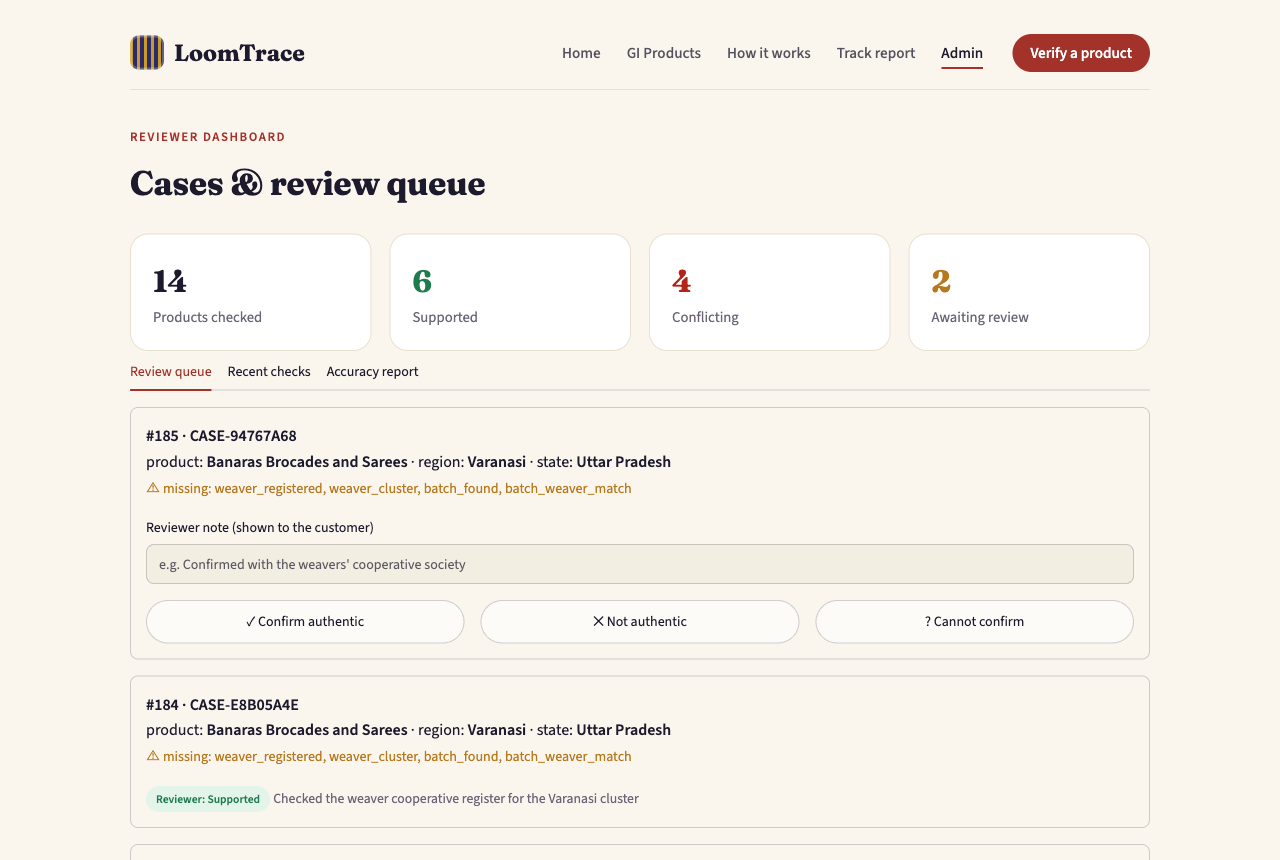
\includegraphics[width=0.8\linewidth]{figures/ui_admin.png}
\caption{Reviewer dashboard: open case with extracted claim, escalation reason, note field and
decision buttons; below it, an earlier case already decided by a reviewer}
\label{fig:admin}
\end{figure}

\begin{figure}[H]
\centering
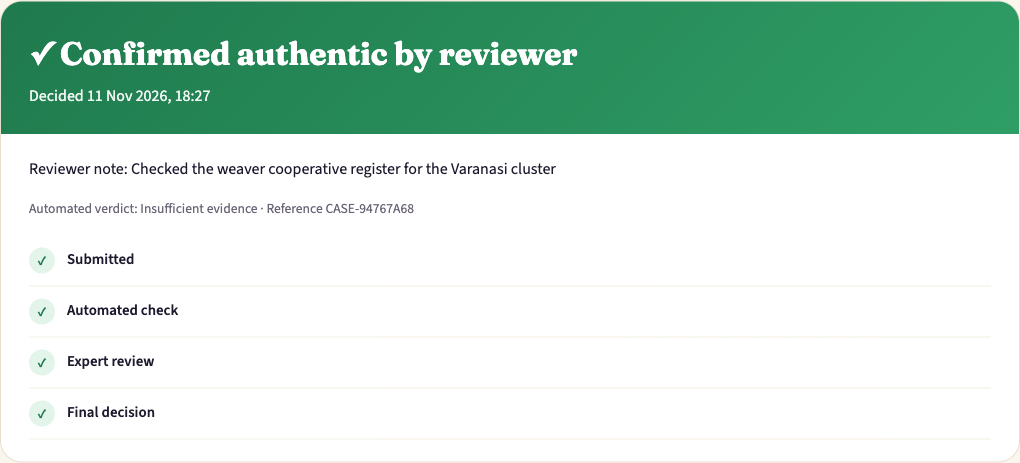
\includegraphics[width=0.5\linewidth]{figures/ui_track.png}
\caption{Requester's view of an escalated case after the reviewer's decision, with the reviewer's
note, the automated verdict and the progress of the case}
\label{fig:track}
\end{figure}

\paragraph{Multi-agent collaboration (partial).} Gathering evidence and judging it are performed by two
separate nodes, the retriever agent and the verifier agent, and the graph's conditional routing acts as
a supervisor. Both nodes are deterministic in the configuration evaluated, so this is a division of
responsibilities rather than a collaboration of independent model-driven agents.

\paragraph{Memory (partial).} Each case has its own memory: the CaseState accumulates the evidence and
trace of every iteration, the checkpoint table preserves each intermediate state, and the case history
and decision tables keep the outcome. There is no memory across cases; for example, the system does
not learn that a particular seller's claims are frequently escalated.

\paragraph{Durable workflow (partial).} Because the full state is written after every node, a case can be
inspected and re-checked at any later time, and human review proceeds asynchronously through the queue.
However, the graph does not automatically resume an interrupted run from its last checkpoint; a run
that is interrupted is re-executed from the start.

\paragraph{Experimentation.} Chapter~8 reports a controlled A/B experiment in which the re-planning loop
is disabled while all other factors are held fixed.
